\cotefile{129}
\scanpage{77}
% archive foliation: 76

$\overline{\mathrm{I}},\overline{\mathrm{II}}$

Vecteurs de Witt

et \unsure{théorie} de

Dieudonné
\scanpage{78}
% archive foliation: 77

I\quad Rappels sur les vecteurs de Witt et \inserted{II} la théorie de Dieudonné.

III\quad Généralités sur les groupes de BT.

\deleted{\unsure{II|IV}}\inserted{IV}\quad Généralités sur les puiss. div. et les cristaux.

\deleted{\unsure{III}}\inserted{V}\quad Foncteur de Dieudonné sur base $\pm$ quelconque: programme \unsure{préliminaire}\inserted{\uline{\unsure{(}et problèmes}}

\deleted{IV}\inserted{VI}\quad F-cristaux. Un théorème de spécialisation pour les groupes de BT.
\scanpage{80}
% archive foliation: 79
\margin{$\overline{\mathrm{I}}$ et $\overline{\mathrm{II}}$}

Rappels sur \deleted{sur}la théorie de Dieudonné (sur corps parfait k).

\margin{\uuline{Serre}, \uline{Corps Locaux}\\
\uuline{Demazure--Gabriel} Schémas en Groupes}

1. Rappels sur vecteurs de Witt.

\margin{$p$ est premier fixé dans tout le cours}

$\underline{W}_n\inserted{(n\geq1)}$, $\underline{W}$ schémas en anneaux sur $\underline{Z}$, $\underline{W}=\varprojlim\underline{W}_n$, avec
$\underline{W}_n=\underline{E}^{n}$ (absolu) comme schéma, $\underline{W}=\underline{E}^{\underline{N}}$ comme schéma, morphismes de transition
\[
R_n:\underline{W}_{n+1}\longrightarrow\underline{W}_n,\quad
R_n(x_1,\ldots,x_{n+1})=(x_1,\ldots,x_n)
\]
Structures additive et multiplicative caractérisées\deleted{p} par la condition que les \deleted{homo}morphismes de schémas
\[
\deleted{\unsure{W}}\qquad
\inserted{\Phi=(\Phi_1,\ldots,\Phi_n):}\quad
\underline{W}_n\longrightarrow\underline{O}^{\inserted{n}}\quad
(=\underline{E}^{\inserted{n}}\text{ comme schéma})
\]
donnés par'
\[
\phi_i(x_1,\ldots,x_n)=\phi_i(x_1,\ldots,x_i)
=x_1^{p^{i-1}}+px_2^{p^{i-2}}+\cdots+p^{i-1}x_i
\]
soi\deleted{en}t \deleted{des}\inserted{\unsure{un}} homomorphisme\deleted{s} d'\deleted{a}\inserted{A}nneaux.

\deleted{Homo}M\uline{orphismes remarquables:} \inserted{Morphisme \uline{additif}}
\[
V_n=V:\underline{W}_n
\xrightarrow[\deleted{\unsure{T}}]{\deleted{\unsure{T}}}\underline{W}_n,\qquad
V(x_1,\ldots,x_n)=(0,x_1,\ldots,x_{n-1})
\]
\deleted{donnés par} d'où par passage à la limite
\[
\deleted{\unsure{R}(x_1,\unsure{\ldots})}\qquad
V:\underline{W}\longrightarrow\underline{W},
\]
puis \deleted{\unsure{morph.}}
\[
\inserted{\text{morphisme d'Anneaux}}\quad
R_n\text{ ou }R:\underline{W}_{n+1}\longrightarrow\underline{W}_n,
\quad R(x_1,\ldots,x_{n+1})=(x_1,\ldots,x_n)
\]
\[
\inserted{\text{morphisme add.}}\quad
\unsure{\Pi|T}_n\text{ ou }\unsure{\Pi|T}:\underline{W}_n\longrightarrow\underline{W}_{n+1},
\quad\unsure{\Pi|T}(x_1,\ldots,x_n)=(0,x_1,,x,x_n)
\]
avec
\[
R_nT_n=V_n,\quad T_nR_n=V_{n+1}.
\]
Enf\unsure{in}\deleted{\unsure{car. p}}, on a
\[
F\text{ ou }F_n:\underline{W}_n\longrightarrow\underline{W}_n,\quad
F(x_1,\ldots,x_n)=(x_1^p,\ldots,x_n^p),
\]
d'où par passage à la limite
\[
F:\underline{W}\longrightarrow\underline{W}
\]
\uline{En caractéristique} $p$
\[
F_{\underline{F}_p}:\underline{W}_{\underline{F}_p}\longrightarrow\underline{W}_{\underline{F}_p}
\qquad(\text{et variante avec }\underline{W}_{n\underline{F}_p})
\]
\scanpage{81}
% archive foliation: 80

est un \uline{homomorphisme d'anneaux} (c'est en effet le Frobenius habituel\deleted{\unsure{)}},
\deleted{et \unsure{on a} $V,D$ sont des \uline{morphismes additifs} (}$V$ est la Verschiebung habituelle) et on a
\[
FV=p.\,\mathrm{id},\quad VF=p.\mathrm{id}\qquad(\text{\uline{en car.} }p).
\]
On introduit aussi le schéma en groupes en
\[
\underrightarrow{W}=\varinjlim_n\underline{W}_n,\quad\text{morphismes de transition du type }D.
\]
Ainsi du point de vue schémas,on a
\[
\underrightarrow{W}=\underline{E}^{(\underline{N})}.
\]
\uline{En car.} $p$, on a commutat\deleted{t}ivité dans
\diagram{\begin{tikzcd}
\underline{W}_n \arrow[r,"T"] & \underline{W}_{n+1}\\
\underline{W}_n \arrow[u,"F"] \arrow[r,"p"] & \underline{W}_{n+1} \arrow[u,"\mathrm{id}"']
\end{tikzcd}}
\deleted{d'où}\inserted{et} commutativité dans
\diagram{\begin{tikzcd}
\underline{W}_n \arrow[r,"T"] \arrow[d,"F^{n-1}"'] & \underline{W}_{n+1} \arrow[d,"F^{n\deleted{\unsure{-1|+1}}}"]\\
\underline{W}_n \arrow[r,"p"] & \underline{W}_{n+1}
\end{tikzcd}},
d'où un homomorphisme canonique
\[
u:\underrightarrow{W}_{\inserted{\underline{F}_p}}\longrightarrow
\varinjlim(\underline{W}_{n\inserted{\underline{F}_p}},p),
\]
qui \deleted{est un} induit un isomorphisme sur les points à valeurs dans un \deleted{corps}\inserted{anneau} parfait.

Soit maintenant $k$ un corps parfait de car. $p$. Alors
\[
W=\underline{W}(k)=\varprojlim W_n\qquad(W_n=\underline{W}_n(k))
\]
est un anneau de valuation discrète de corps résiduel \deleted{\unsure{k, dit}} $W_1=k$, d\deleted{e}'idéal maximal engendré par $p$, et de corps des fractions
\[
K=W[1/p]
\]
de caractéristique nulle. L'homomorphisme $u$ précédent induit un isomorphisme de groupes
\[
u:\underrightarrow{W}(k)\xrightarrow{\sim}K/W.
\]
On va introduire sur $\unsure{\underline{W}|\underrightarrow{W}}_k$ une structure de schéma en groupes avec
\scanpage{82}
% archive foliation: 83

Si $k$ est un corps parfait, ceci donne une décomposition canonique en somme directe
\[
G\simeq G_{\mathrm{et}}\times G_{\mathrm{mult}}\times G_{\mathrm{bi}}
\]
et la catégorie des $G$ est can. \unsure{isomorphe} au produit des trois catégories correspondantes.

$G_{\mathrm{et}}$ et $G_{\mathrm{mult}}$, structure connue par théorie de Galois

$G_{\unsure{\mathrm{uni}|\mathrm{bi}}}$ ? Donné par théorie de Dieudonné.

\diagram{\begin{tikzcd}[column sep=small,row sep=small]
& \unsure{f_G} & |[draw,ellipse]|\text{nilpotent} \arrow[r,Leftrightarrow] \arrow[dll,no head,bend right=30] & G_{\mathrm{et}}=0\quad\text{i.e. }G^*\text{ unipotent} & f_G\text{ isom}\Longleftrightarrow G\text{ étale}\\
\parbox{3cm}{\margin{préciser que ça veut dire, en introduisant Frob. et Versch. \uline{itérés}.}} & w_G & |[draw,ellipse]|\text{nilpotent} \arrow[r,Leftrightarrow] \arrow[ll,no head,bend left=20] & G_{\mathrm{mult}}=0\quad\text{i.e. }G\text{ unipotent} & w_G\text{ isom}\Longleftrightarrow G\text{ d.m.}
\end{tikzcd}}

4. \uline{Théorie de Dieudonné}: \uline{le th. d'équivalence}.

On donne $k$ corps parfait de car. $p>0$

La théorie de Dieudonné fournit une \inserted{anti}équivalence
\diagram{\begin{tikzcd}[column sep=large]
p\text{-}\mathrm{Gr}_{\unsure{f}}(k) \arrow[r,"\approx"] &
\left\{\begin{array}{l}
\text{Catégorie des modules de longueur}\\
\text{finie }M\text{ sur }W,\text{ munis de}\\
F_M,V_M:M\mathbin{\unsure{-|\longrightarrow}}M\text{ satisfaisant}\\
F\lambda=\lambda^\sigma F,\quad\lambda V=V\lambda^\sigma\\
FV=p.\mathrm{id},\qquad FV=p.\mathrm{id}
\end{array}\right.\\
G \arrow[r,mapsto] & D^*(G)
\end{tikzcd}}

\uline{Interprétation}:
\diagram{\begin{tikzcd}
M^\sigma \arrow[r,shift left,"F_M"] & M \arrow[l,shift left,"V_M"]
\end{tikzcd}}

De plus, \unsure{\ldots}\ \deleted{\unsure{on a}}\deleted{\unsure{d'ici}} compte tenu que $D^*$ commute au changement de base, donc $D^*(G^{(p)})\simeq D^*(G)^{(p)}$ :
\[
F_{D^*(G)}=D^*(f_G),\qquad V_{D^*G}=D^{\unsure{*}}(w_G)
\]
d'où le dictionnaire :
\diagram{\left\{\begin{array}{lll}
G\text{ unipotent}&\Longleftrightarrow&V_M\text{ nilpotent}\\
G^*\text{ \unsure{unipotent}}&\Longleftrightarrow&F_M\text{ \unsure{unipotent|nilpotent}}\\
G\text{ étale}&\Longleftrightarrow&F_M\text{ isom}\\
G^*\text{ étale}&\Longleftrightarrow&V_M\text{ isom}\\
\text{i.e. }G,\text{ gr. d.m.}&&
\end{array}\right.}
\scanpage{83}
% archive foliation: 84

$\overline{\mathrm{III}}$\quad Propriétés

Générales

des B.T.
\scanpage{84}
% archive foliation: 85

Exemples de groupes de BT.

a)\quad Soit $G$ un schéma en groupes lisse sur $S$, \deleted{à fibres connexes} extension d'un schéma abélien\inserted{$A$} par un tore\inserted{$T$}. Alors $p.\mathrm{id}_G$ est un épimorphisme, et les $G(n)=\operatorname{Ker}p^n\mathrm{id}_G$ sont des groupes finis localement libres (commencer par cas d'un schéma abélien). Donc $G(\infty)=\lim G(n)$ est un groupe de BT.\inserted{Si $A$ ($T$) de dim relative $a(m)$, $G(\infty)$ de rang $2a+m$.} Cas important: $\mu\deleted{\unsure{(\infty)}}=\underline{G}_m(\infty)$.

b)\quad Supposons que $S$ soit \deleted{à caractéristique résiduelle égale à $p$}\inserted{tel que $p$ soit loc. nilpotent sur $S$.} et soit $G$ un groupe \inserted{de Lie}formel sur $S\deleted{\unsure{x}}$ (cette notion sera précisée plus tard, pour ceux qui ne la connaitraient pas encore \ldots).\inserted{On a alors $G=G(\infty)=\lim G(n)$.} Supposons que $p.\mathrm{id}_G$ soit un épimorphisme; lorsque $S$ est artinien local, comme unique point $s\in S$, l'hypothèse revient à dire que $p.\mathrm{id}_{G_s}$ dans $G_s$ est un épimorphisme, ou encore que $G_{\bar{s}}$ ne contient pas de sous-groupe de Lie formel isomorphe à $\underline{G}_a$. (Mais si $S$ n'est pas réduit à un point, p. ex. si $S$ est un trait, la condition que $p.\mathrm{id}_G$ soit un épimorphisme \uline{n'est pas} une simple condition fibre par fibré. Prendre par exemple le groupe de Lie formel associé à\deleted{un groupe} la courbe ell\deleted{\unsure{e}}iptique modulaire, au voisinage d'un point de Hasse nul ..\inserted{$(\unsure{\dagger|*})$}) Il devrait être vrai que \deleted{les} $G(1)$ dont les $G(n)$ sont finis localement libres (plus généralement, si on a un épimorphisme de groupes de Lie formels de même dimension relative, le noyau devrait être fini localement libre, et réciproquement \ldots). C'est en tous cas le cas si $S$ est artinien; supposons cette condition supplémentaire vérifiée. On trouve alors \inserted{que $G$ est}un groupe de BT \deleted{$G(\infty)$}. De plus, les $G(n)$ sont radiciels, et on \inserted{prouvera par la suite que l'}trouve une équivalence entre la catégorie des groupes de BT $G$ sur $S$ tel que $G(1)$ soit radiciel (ou ce qui revient au même, les $G(n)$ le soient -- on dit alors que $G$ est à fibres connexes), et la catégorie des groupes de Lie formels \inserted{$G$}sur $S$ tels que $p.\mathrm{id}_G$ soit un épimorphisme et tel que $G(1)$ soit fini localement libre (ces deux

\margin{$(\unsure{\dagger|*})$ La condition suppl. à rajouter devrait être : fibres de ``hauteur'' localement constante}
\scanpage{85}
% archive foliation: 86

conditions supplémentaires étant sans doute équivalentes).\inserted{Le rang de $G$ comme groupe de BT s'appelle la \uline{hauteur} du groupe formel.}

c)\quad Groupes de BT ind-étales: par $G\quad T_p(G)$, \deleted{ces} la catégorie en question équivaut à celle des faisceaux $p$-adiques (étales) contants tordus \deleted{locale} sans torsion; si $S$ est connexe muni d'un point géométrique $\bar{s}$, cette catégorie équivaut à celle des représentations continues de $\pi_1(S,\bar{s})$ par des modules libres de type fini sur $\underline{Z}_p$.

Groupes de BT de t.m. ou ``\unsure{toroidaux|toroïdaux}'' : si $G(1)$, donc les $G(n)$, sont de type multiplicatif. Associant à un tel $G$ le système projectif des $G(n)^*$, on trouve \deleted{encore} une \inserted{anti}équivalence entre cette catégorie et la catégorie des faisceaux $p$-adiques constants tordus sans torsion. Composant avec le foncteur $F\mapsto F^{\inserted{\vee}}$, on trouve une équivalence au lieu d'une antiéquivalence, qui peut aussi s'expliciter comme \deleted{$G\mapsto\underline{\operatorname{Hom}}_{\mathrm{gr}}(\unsure{\mu_n},G)$}
\[
G\longmapsto\underline{\operatorname{Hom}}_{\mathrm{gr}}(\mu,G)
\overset{\mathrm{dfn}}{=}
\bigl(\underline{\operatorname{Hom}}_{\mathrm{gr}}(\mu(n),G(n))\bigr)_{n\geq1}.
\]
\margin{\unsure{k}}
\begin{center}(abus de notation)\end{center}
Noter que si les car. rés. sont $p$, alors les groupes de BT tor\deleted{\unsure{t}}oidaux sont \deleted{infinitésimaux} à fibres connexes (et réciproquement\inserted{s'il en est ainsi, car. rés sont $p$}).

d)\quad Groupes de BT comme extension d'un groupe ind-étale par un groupe de Lie formel.

Supposons d'abord $S$ \deleted{artinien (\unsure{ou}} réduit à un point\inserted{$s$}. Alors pour tout groupe fini $H$ sur $S$, $H^o$ est un sous-groupe, dépendant fonctoriellement de $H$. Si $H$ est fini localement libre, de même $H^o$, et $H/H^o$ est \deleted{\unsure{de}} un groupe fini localement libre (cf. SGA 3 $\mathrm{VI}_A$ \ldots), qui est étale. Ainsi $H$ s'écrit canoniquement et fonctoriellement comme extension d'un groupe étale par un groupe infinitésimal (tout fini localement libre). Si $k(s)$ est de car. $p\quad0$, alors procédant par dualité, on trouve un sous-groupe $G^{\mathrm{tm}}$ de $G^o=G^{\mathrm{inf}}$, qui est le plus grand sous-groupe de t.m de $G$, d'où une filtration à trois crans (qu'on avait eu le tort de ne définir précédemment que sur un \uline{corps} \deleted{de} de base). Passant maintenant à la
\scanpage{86}
% archive foliation: 87

limite\inserted{pour les $G(n)$}, on voit que tout groupe de BT $G$ sur $S$ \deleted{est extension d'un groupe de BT $\unsure{G(}\quad G^o\overset{\mathrm{dfn}}{=}\lim G(n)$} admet une filtration par des sous-groupes de BT $G^o=\lim G(n)^o$ (plusgrand sous-groupe de BT à fibres connexes) et\inserted{(si car. $k(s)=p$) par} $G^{\mathrm{tm}}=\lim G(n)^{\mathrm{tm}}$ (plus grand sous-groupe de BT \deleted{à fibres} toroidal), canonique et \unsure{fonctorielle|foncturielle} en $G$. En particulier, il est extension d'un groupe de BT ind-étale $G/G^o$ par le groupe de BT à fibres connexes $G^o$, qui peut s'interpréter (si $k(s)$ de car. $p$ \deleted{)comme} et l'idéal maximal de $\underline{O}_{S,s}$ nilpotent, p.ex. $S$ noethérien) comme un groupe de Lie formel, et il pourra même s'interpréter comme extension triple d'un\deleted{e} ind-étale par un connexe unipotent par un toroidal.

Sur une base non ponctuelle (p.ex. un trait de car. $p$ )\deleted{0)}, il n'est plus vrai en général qu'un groupe de BT $G$ \deleted{admette} soit extension d'un groupe de BT ind-étale par un groupe de BT à fibres connexes. Il suffit encore de prendre le groupe \deleted{$\unsure{G(\infty)}$} $A(\infty)$, $A$ courbe elliptique modulaire en car. $p$ : l'ennui provient encore des points où $A_s$ est d'invariant de Hasse nul. On a la

\uline{Proposition}.\quad Conditions équivalentes sur le groupe de BT $G$ sur $S$:

(i)\quad $G$ est extension d'un groupe de BT ind-étale par un groupe de BT à fibres connexes.

(ii)\quad Pour tout $n$, $G(n)$ est extension d'un groupe fini étale par un groupe fini radiciel.

(iii)\quad Kif-kif avec $n=1$.

(iv)\quad La fonction $s\mapsto\operatorname{rang\ Sép}G_s=\operatorname{card}G(\bar{s})$ est localement constante.

Résulte facilement du résultat suivant (qui figure dans EGA IV ?):

\uline{Lemme}.

Si $\unsure{X}\longrightarrow S$ est un morphisme fini localement libre, alors $X\longrightarrow S$ se facto-
\scanpage{87}
% archive foliation: 88

rise en un morphisme \deleted{radiciel} étale suivi d'un morphisme radiciel\inserted{\unsure{surjectif}} sss la fonction $s\mapsto\operatorname{rang\ sép}G_s$ est localement constante. La factorisation obtenue est alors unique et fonctorielle en $G$, \deleted{et les facteurs qui y \unsure{int} interviennent $G^{\mathrm{ét}}$ et $G^o$ \unsure{s}} (d'où résulte que si $G$ est un schéma en groupes, la factorisation est une structure d'extension de groupes; de plus $G^{\mathrm{ét}}$ et $G^o$ sont alors foncteurs exacts en $G$ pour suites exactes courtes\deleted{\unsure{.}}).
\scanpage{88}
% archive foliation: 89

\uline{Proposition}\quad (i) Toute extension d'un groupe de BT par un autre est un groupe de BT.

(ii)\quad Pour tout monomorphisme de groupes de BT, le conoyau est de BT.

\deleted{(iii)\quad Pour tout épimorphisme de groupes de BT, le noyau est de BT.}

\deleted{En d'autres termes,} Si on a une suite exacte courte
\[
0\unsure{\longrightarrow|-}G'\longrightarrow G\longrightarrow G''\longrightarrow0
\]
\deleted{avec deux des termes de BT, le troisième l'est} On a une suite exacte
\[
0\longrightarrow G'(1)\unsure{-|\longrightarrow}G(1)\unsure{-|\longrightarrow}G''(1)\longrightarrow G'/pG'
\longrightarrow\bigl[G/pG\longrightarrow G''/pG''\longrightarrow0\bigr]
\]
qui dans les deux cas \unsure{enfisagés|envisagés} montre qu'on a
\[
0\longrightarrow G'(1)\unsure{-|\longrightarrow}G(1)\unsure{-|\longrightarrow}G''(1)\longrightarrow0,
\]
d'où le fait que $G(1)$ (resp. $G''(1)$) est fini loc. libre. D'autre part il est clair que $G$ (resp. $G''$) est $p$-divisible et de $p$-torsion, cqfd.

\uline{Rang ou hauteur} d'un groupe de BT. Le rang de $G(1)$ est de la forme $p^{\unsure{r|n}}$ en chaque point ($\unsure{r|n}$ une fonction localement constante sur $S$). On appelle $r$ le \uline{rang} ou la \uline{hauteur} du groupe de BT. On notera que $G(n)$ est de rang $p^{rn}$.
\scanpage{90}
% archive foliation: 91
2. Sur certains schémas en groupes finis loc. libres en car. $p$.
\inserted{Applications aux BT}

\uline{Proposition} 2.1. Cf. prop.14 des Notes I

\uline{Proposition} 2.2. Cf. prop.1 des Notes I, en introduisant la notation
$G[i]=\operatorname{Ker}\underline f_G^i$. Fixant $i$ avec
$1\leq i\unsure{<|\leq}n-1$, on a équivalence (si $G=G(n)$):

(i) $\underline f_G^i:G\longrightarrow G[n-i]^{p^{n-i}}$ est plat (donc fid. plat).

(i bis) L'homomorphisme précédent est couvrant.

\deleted{(ii) Les groupes $G_{\unsure{j|i}}$ sont tous plats, (donc loc. libres) sur $S$,}

(ii) Gradué associé: point de vue \inserted{\unsure{f|F}}aisceautique

(ii bis) Gradué associé: point de vue schémas en groupes.

\[\unsure{f^{\,i}=-\!\!-\!\!-\!\!-}\]

NB Un tel groupe est lisse à l'ordre $p^n-1$. Conjugant 2.1 et 2.2, on trouve donc:

\margin{$G[n]\overset{\mathrm{dfn}}=G(n)[n]=G(i)[n]\quad\text{pour }i\geq n$}
\uline{Corollaire} 2.3. Soit $G$ un groupe de BT sur $S$ de car. $p$ \deleted{$\unsure{>0}$}.
Alors pour \deleted{\unsure{tous}}
tout entier $n\inserted{>}0$, $G(n)$ est lisse à l'ordre \deleted{$\unsure{n}$}\inserted{$p^n-1$} sur $S$, et on a
$\operatorname{Inf}^k(G)\subset G[n]$ pour $k\leq p^n-1$.
\margin{$\subset G[n]$}

\deleted{\unsure{3}}
Comme corollaire de 2.2 \deleted{et de 1.4}, on trouve:

\deleted{\uline{Corollaire}}\inserted{\uline{Proposition}} 2.4. La catégorie des groupes de Lie formels (comm)\inserted{$G$} sur $S$ de car $p$ est équivalente à la catégorie des systèmes inductifs $\underline f$-coadiques de schémas en groupes finis localement libres $G[n]$ sur $S$ satisfaisant les conditions équivalentes de 2.2.

Conjug\inserted{u}ant avec 2.3, on trouve:

\deleted{\uline{Proposition}}\inserted{\uline{Théorème}} 2.5. Soit $G$ un groupe de BT sur $S$ de car.$p$. Alors on a
\[
\bar G\overset{\mathrm{dfn}}=\operatorname{Inf}^{\infty}(G)=\varinjlim G(n)[n]
\]
est un groupe de Lie formel sur $S$ tel que $\bar G[n]=G(n)\unsure{(|[}n]$. Pour $k\leq p^n-1$, on a
\[
\operatorname{Inf}^kG=\operatorname{Inf}^k\bar G\quad\deleted{\unsure{=G(n}}=\operatorname{Inf}^kG(n)\subset G(n)[n]\subset G(n).
\]
\diagram{\begin{array}{c}G(n)[n]\\\Vert\\G[n]\\\Vert\\\bar G[n]\end{array}}
\margin{\figure{\begin{tikzpicture}\node[draw,ellipse,rotate=55,align=center]{donner\\relation\\$d+d^{\unsure{t|*}}=h$};\end{tikzpicture}}}
\scanpage{91}
% archive foliation: 92
4. \deleted{\unsure{Théorè}} \uline{Déformations de groupes de} BT : \uline{énoncés}.

Le résultat principal, qui sera essentiel pour la théorie de Dieudonné est le suivant(cf lettre Illusie, 6.4):

\uline{Théorème} 4.1. Soit $S_o\hookrightarrow S$ une nilimmersion, avec $S$ affine, $G_o$ un groupe de BT sur $S_o$. Alors:

a) Il existe un groupe de BT $G$ sur $S$ qui prolonge $G_o$.

b) Lapplication
\[
(*)\qquad E(G_o,S)\longrightarrow E(G_o(n),S)
\]
est surjective\unsure{;|.}

c) Si $i$ est nilpotente d'ordre $k$ et si $p^N1_{S_o}=0$, alors l'application $(*)$ est bijective pour $n\geq kN$.

d) Si de plus $k=1$, alors $E(G_o,S)$ est un torseur sous $\underline t^{\deleted{\unsure{*}}}_{G_o^*}\otimes t_{G_o}$.

Ce résultat s'obtient via un résultat de déformation pour les groupes de BT tronqués (je ne sais pas procéder directement !).

5. \uline{Rapport sur le complexe cotangent relatif}.
\scanpage{92}
% archive foliation: 93
\uline{Complexe cotangent relatif.}

\figure{\begin{tikzpicture}\node[draw,ellipse]{$A$};\end{tikzpicture}}
Définition \unsure{admise} $L_\bullet^{X/Y}$ ``dérivé'' du foncteur $\Omega^1_{X/Y}$

Fonctorialité.

Calcul tronqué $\tau_{\leq1}(L_\bullet^{X/Y})$ par immersion dans form\unsure{\textsuperscript{t}} lisse

\unsure{Quasi-éléments|Quasi-étales}, \unsure{critères|extensions}

Cas intersection complète relative: $H_i(L_\bullet^{X/Y})=0$ si $i\geq2$.

Triangle exact de transitivité et suite exacte longue associée

Changement de base
\diagram{\begin{tikzcd}X\arrow[d,"f"]&X'\arrow[l]\arrow[d,no head]\\S&S'\arrow[l,"g"']\end{tikzcd}}
dans le cas $\underline{\operatorname{Tor}}_i^{\unsure{\mathcal O_S|\mathcal O}}(\underline O_X,\mathcal O_{\unsure{S'}})=0$ pour $i>0$ (p.ex $f$ \uline{ou} $g$ plats)

\uline{Application 2}\quad Prolongement de morphismes
\diagram{\begin{tikzcd}X\arrow[d,no head]&Y_o\arrow[l,"f_o"']\arrow[d,hook]\\S&Y\arrow[l]\arrow[ul,dashed,"f?"']\end{tikzcd}}
$Y_o=V(J),\ J^2=0$

a) Obstruction dans $\operatorname{Ext}^1_{\underline O_{Y_o}}(\unsure{\mathbf L}f_o^*(L_\bullet^{X/S}),J)$

b) Indéterminations dans $\operatorname{Ext}^0_{\underline O_{Y_o}}(\mathbf Lf_o^*(L_\bullet^{X/S}),J)$

\uline{Application 1}
\diagram{\left\{\begin{array}{l}
\operatorname{\unsure{Ext|Exal}}_{\underline O_S}(\underline O_X,J)\simeq\operatorname{Ext}^1_{\underline O_X}(L_\bullet^{X/S},J)\\
\text{autom. d'une extension}\simeq\operatorname{Ext}^0_{\underline O_X}(L_\bullet^{X/S},J)=\operatorname{Hom}(\Omega^1_{X/S},J)
\end{array}\right.}

\uline{Application 3}\quad Déformations plates
\diagram{\begin{tikzcd}X_o\arrow[d]&X?\arrow[l,dashed]\arrow[d,dashed]\\S_o\arrow[d,equal]&S\arrow[l]\\V(J),\ J^2=0&\end{tikzcd}}

a) Obstruction à déformer
\[
\in\operatorname{Ext}^2_{\underline O_{X_o}}(L_\bullet^{X_o/S_o},J\otimes_{\mathcal O_{S_o}}\mathcal O_{X_o})
\]
b) Indéterminations pour \unsure{déformer}
\[
\in\operatorname{Ext}^1_{\mathcal O_{X_o}}(L_\bullet^{X_o/S_o},J\otimes_{\underline O_{S_o}}\mathcal O_{X_o})
\]
\diagram{\begin{tikzcd}[column sep=large]&\text{b)}\arrow[dl]\\\text{lien avec Ex.2}&\end{tikzcd}}

c) Autom. d'une déform.\unsure{\textsuperscript{tion}}
\[
\operatorname{Ext}^0_{\mathcal O_{X_o}}(L_\bullet^{X_o/S_o},J\otimes_{\mathcal O_{S_o}}\mathcal O_{X_o})
\]
\scanpage{93}
% archive foliation: 94
\figure{\begin{tikzpicture}\node[draw,ellipse]{$B$};\end{tikzpicture}}
Cas des groupes (commutatifs pour fixer les idées) \uline{plats}.

\margin{introduit par \unsure{Mazur-Robert}}
On pose
\diagram{\begin{array}{lll}
\ell_\bullet^{G/S}=\mathbf Le^*(L_\bullet^{G/S})&&\text{complexe de co-Lie}\\
\overset{\vee}{\ell}_\bullet^{G/S}=R\underline{\operatorname{Hom}}(\ell_\bullet^{G/S},\underline O_S)&&\rule{3cm}{0.3pt}\ \text{Lie}
\end{array}}
\margin{\uline{variances}}

Si $G$ est \uline{loc. de prés. finie} sur $S$, il est d'int. complèt rel. et on a
\diagram{\left\{\begin{array}{lll}
\ell_\bullet^{G/S}&\text{parfait d'ampl. parfaite}&\subset[-1,0]\\
\overset{\vee}{\ell}_\bullet^{G/S}&\rule{5cm}{0.3pt}&\subset[0,1]
\end{array}\right.}

Notations
\deleted{$\unsure{\underline\omega_G,\underline n_G}$}
\diagram{\left\{\begin{array}{l}
\underline\omega_G=\underline H_0(\ell_\bullet^{G/S})\\
\underline n_G=\underline H_1(\ell_\bullet^{G/S})\\
\underline t_G=H^0(\overset{\vee}{\ell}_\bullet^{G/S})\\
\nu_G=H^1(\overset{\vee}{\ell}_\bullet^{G/S})
\end{array}\right.\qquad t_G=\overset{\vee}{\omega}_G,\quad\underline n_G=\overset{\vee}{\nu}_G}
\[
\operatorname{rg}\ell_\bullet^G=\dim G\qquad(=\operatorname{rg}\underline\omega_G-\operatorname{rg}n_G\ \text{quand }\underline\omega_G,\underline n_G\text{ sont loc. libres}).
\]

Suite exacte de transitivité: Une suite exacte
\[
0\longrightarrow G'\longrightarrow G\longrightarrow G''\longrightarrow0
\]
de schémas en groupes plats implique une suite exacte
\diagram{\begin{tikzcd}&\ell_\bullet^{G'}\arrow[dl,"1"',very thick]&\\
\ell_\bullet^{G''}\arrow[rr]&&\ell_\bullet^G\arrow[ul]
\end{tikzcd}\quad\unsure{0}}
,
d'où, si $G'$ loc. de prés. finie, suite exacte courte
\[
0\longrightarrow n_{G'}-n_G\longrightarrow n_G\longrightarrow\omega_{G''}-\omega_G-\omega_{G'}-0.
\]

Formule \uline{remarquable}
\[
\boxed{R\underline{\operatorname{Hom}}(\ell_\bullet^G,J)\simeq\tau_{\leq1}R\operatorname{Hom}(G^{\unsure{*}},J)}
\]
\margin{\uuline{Faisant} $J=\underline O_S$, $G\mapsto G^*$, \uline{\unsure{à vérifier !}}
\diagram{\left\{\begin{array}{l}
\underline{\operatorname{Hom}}(G^*,\underline O_S)\simeq\underline t_{G^*}\\
\underline{\operatorname{Ext}}^1(G,\underline O_S)\simeq\underline\nu_G
\end{array}\right.}}
\scanpage{94}
% archive foliation: 95
\uline{Lien avec théorie de Dieudonné} (sur corps parfaits)

Si $D^*(G)=M$, on aura
\diagram{\begin{tikzcd}[column sep=small]
0\arrow[r]&({}_FM)^{\unsure{\varphi|\sigma}}\arrow[r,no head]\arrow[d,phantom,"\unsure{\wr|\Vert}"]&({}_pM)^{\varphi}\arrow[r,"F"]\arrow[d,phantom,"\unsure{\wr|\Vert}"]&{}_VM\arrow[r,no head]\arrow[d,phantom,"\unsure{\wr|\Vert}"]&M_F\arrow[r,"V"]\arrow[d,phantom,"\unsure{\wr|\Vert}"]&(M_p)^{\varphi}\arrow[r,no head]\arrow[d,phantom,"\unsure{\wr|\Vert}"]&(M_V)^{\varphi}\arrow[r,no head]\arrow[d,phantom,"\unsure{\wr|\Vert}"]&0\\
0\arrow[r]&\underline n_G\arrow[r,very thick]&D^*_{\inserted{p}}(G^*)^{\vee}\arrow[r,no head]&t_{G^*}\arrow[r]&\omega_G\arrow[r]&D^*_{\inserted{p}}(G)\arrow[r]&\nu_{G^*}\arrow[r,no head]&0
\end{tikzcd}},

en fait on aura
\diagram{\begin{array}{ccc}
\ell_\bullet^G\simeq&\mathbb D/F\mathbb D&\overset{\mathbf L}{\otimes}_{\mathbb D}M\\
&\Vert&\\
&k_{\unsure{\sigma|o}}[V]&
\end{array}}
et un isom de \unsure{triangles} \unsure{exacts}
\diagram{\begin{tikzcd}
&\overset{\vee}{\ell}_\bullet^{G^*}\arrow[dl,"?"']&\\
\ell_\bullet^G[-1]\arrow[rr]&&\Delta^{\unsure{*|\alpha}}(G)\arrow[ul]
\end{tikzcd}}
et
\diagram{\begin{tikzcd}
&\mathbb D/V\mathbb D\overset{L}{\otimes}_{\mathbb D}M\arrow[dl,"1"']&\\
\mathbb D/F\mathbb D\overset{L}{\otimes}_{\mathbb D}M\arrow[rr]&&\mathbb D/p\mathbb D\overset{\mathbf L}{\otimes}_{\mathbb D}M\arrow[ul]
\end{tikzcd}}

Le triangle de gauche, avec un $\Delta^{\unsure{*|\alpha}}(G)$ d'ampl. parfaite $\subset[0,1]$, devrait exister sur \uline{toute} base.
\scanpage{95}
% archive foliation: 96
\figure{\begin{tikzpicture}\node[draw,ellipse]{$C$};\end{tikzpicture}}
\uline{Application aux déformations de groupes \inserted{comm.} plats} (Deligne-Illusie)

\inserted{\figure{\begin{tikzpicture}\node[draw,ellipse]{$\unsure{0}$};\end{tikzpicture}}
Déformations de torseurs sous groupes plats de \uline{prés. finie}
$\operatorname{Ext}^0(\unsure{\ell_\bullet^G},J),\quad\operatorname{Ext}^1(\ell_\bullet^G,J)$}

\margin{cf ma lettre à Illusie}
\figure{\begin{tikzpicture}\node[draw,ellipse]{$1$};\end{tikzpicture}}
Prolongement d'homomorphismes de groupes plats
\diagram{\begin{tikzcd}G_o\arrow[rr,"u_o",no head]\arrow[dr,no head]&&H_o\arrow[dl]\\&S_o&\end{tikzcd}\qquad
\begin{tikzcd}G\arrow[rr,dashed,"u?"]\arrow[dr,no head]&&H\arrow[dl,no head]\\&S&\end{tikzcd}}

a) Obstruction dans $\operatorname{Ext}^1_{\deleted{\unsure{\mathcal O}}\inserted{\mathbf Z}}(G_o,\overset{\vee}{\ell}_\bullet^{H_o}\overset{\mathbf L}{\otimes}_{\mathcal O_S}J)$

b) Indéterminations dans $\operatorname{Ext}^0_{\deleted{\unsure{\mathcal O}}\inserted{\mathbf Z}}(G_o,\overset{\vee}{\ell}_\bullet^{H_o}\overset{\mathbf L}{\otimes}_{\mathcal O_S}J)$

\figure{\begin{tikzpicture}\node[draw,ellipse]{$2$};\end{tikzpicture}}
Déformations de groupes plats
\diagram{\begin{tikzcd}G_o\arrow[d,no head]&G?\arrow[l,no head]\arrow[d,no head]\\S_o&S\arrow[l]\end{tikzcd}}

a) Obstruction dans $\operatorname{Ext}^2_{\mathcal O_{S_o}}(G_o,\overset{\vee}{\ell}_\bullet^{G_o}\overset{\mathbf L}{\otimes}J)$

b) Indétermination dans $\operatorname{Ext}^1_{\mathcal O_{S_o}}(\quad,\quad)$

c) Autom. d'un relèvement: $\operatorname{Ext}^0_{\mathcal O_{S_o}}(\quad,\quad)=\operatorname{Hom}(G_o,\ )$
\inserted{($\underline{\operatorname{Hom}}(\underline\omega_{G_o},J)$)}

Variante pour $\unsure{\Lambda}$-modules

\figure{\begin{tikzpicture}\node[draw,ellipse]{$D$};\end{tikzpicture}}
\uline{Cas des groupes de} BT \uline{tronqués}.
\inserted{(Lettre Illusie 5.3)}

\uline{Prop.} $G(n)$ B.T. tronqué, $p^N.1_S=0$, \uline{pour} $n\unsure{\geq|=}N$.
\figure{\begin{tikzpicture}\draw (0,0)--(0,8);\end{tikzpicture}}
\[
\underline\omega_{G(n)}=\underline H_0(\ell_\bullet^{G(n)})\quad\text{et}\quad\underline n_{G(n)}=\underline H_1(\ell_\bullet^{G(n)})
\]
loc libres de $\unsure{\overline m}$ rang. Si $n\geq n'\geq N$, l'inclusion $G(n')\subset G(n)$ \deleted{$\unsure{\simeq}$} induit un \uline{isom}
\[
\underline\omega_{G(n)}\simeq\underline\omega_{G(n')}
\]
et si: $n'\leq n-N$, l'hom \uline{nul}
\[
\underline n_{G(n)}\xrightarrow{0}\underline n_{G(n')}
\]
La projection $G(n)\longrightarrow G(n')$ induit
\[
\underline n_{G(n')}\xrightarrow{\sim}\underline n_{G(n)}
\]
et
\[
\underline\omega_{G(n')}\xrightarrow{0}\underline\omega_{G(n)}
\]
On a, si $n\geq2N$\qquad$\underline\omega_{G(n)}\simeq\underline n_{G(n)}$
\scanpage{96}
% archive foliation: 97
\uline{Th} Soit $G=G(n)$ groupe de BT tronqué d'échelon $n$, $M$ un module \unsure{qu. coh.} annulé par $p^n$.
\figure{\begin{tikzpicture}\draw (0,0)--(0,0.7);\end{tikzpicture}}
On a
\diagram{\left\{\begin{array}{l}
\underline{\operatorname{Ext}}^1_{\Lambda_n}(G,M)=0\\
\underline{\operatorname{Ext}}^2_{\Lambda_n}(G,M)\xrightarrow{\sim}\underline{\operatorname{Ext}}^2_{\mathbf Z}(G,M)
\end{array}\right.}

\uline{NB} $\underline{\operatorname{Ext}}^2_{\mathbf Z}(G,M)=0$ si $2$ inv., pour $\forall G$ fini loc. libre; cela simplifie la théorie des déformations pour les BT en car. $p\ne2$ !).
\scanpage{97}
% archive foliation: 98
\unsure{Sotties|Sottises} sur \unsure{Groupes} $p$-divisibles,
et groupes de B.T.
\scanpage{98}
% archive foliation: 99
$\mathcal C$ Catégorie Abélienne

$A$ objet de $\mathcal C$, muni d'un endomorphisme $f$

$n\in\mathbb N^*$, tel que $f^n=0$
\[
\operatorname{gr}_f^i(A)=f^iA/f^{i+1}A
\]
\diagram{\begin{tikzcd}
\theta:\operatorname{gr}_f^0(A)[\unsure{T|\Lambda}]\arrow[r,"\text{\uline{surj}}"']&\operatorname{gr}_f^*(A)
\end{tikzcd}\qquad
\begin{tikzcd}
\theta^i:\operatorname{gr}_f^0(A)\deleted{\unsure{t}}\arrow[r,"\deleted{\unsure{\sim}}","{f^i\atop\text{surj}}"']&\operatorname{gr}_f^i(A)
\end{tikzcd}}

\uline{Conditions équivalentes}

(i) $\theta$ est un isom en degrés $\unsure{<|\leq}n-1$, i.e. $\theta^i$ isom si $\unsure{0}\leq i\leq n-1$.

(i bis) $\theta$ est \uline{injectif} en degrés $<n-1$, i.e. $\theta^i$ injectif pour $\unsure{0}\leq i\leq n-1$

(i ter) $\theta^{n-1}$ est injectif

(ii) $(f^i)^{-1}(f^{i+1}A)=fA$ pour $0\leq i\leq n-1$

(ii bis) \deleted{$\unsure{(f^{n-1})}$} $\boxed{\operatorname{Ker}f^{n-1}=fA}$
\diagram{\begin{tikzcd}\text{(ii bis)}\arrow[d,Rightarrow]\\\text{(iii)}\end{tikzcd}}

(iii) $\operatorname{Ker}f^j=\operatorname{Im}f^{n-j}$ pour \deleted{tout} $0\leq j\leq n$

(iv) $\exists\ \deleted{\unsure{g}}\ j,\quad1\leq j\leq n-1$, tel que $\operatorname{Ker}f^j=\operatorname{Im}f^{n-j}$

\diagram{\begin{tikzcd}
&\text{(ii)}\arrow[r,Rightarrow]\arrow[d,Rightarrow]&\text{(ii bis)}\arrow[d,Rightarrow]\\
\text{(i)}\arrow[r,Leftrightarrow]&\text{(i bis)}\arrow[r,Rightarrow,"\deleted{\unsure{\Leftarrow}}"']&\unsure{\text{(i ter)}}
\end{tikzcd}} trivial

$(\text{i ter})\Longrightarrow(\text{i bis})$ car $\theta^{n-1}=\theta^{\deleted{\unsure{i}}\inserted{n-1-i}}\theta^i$.

\deleted{$(\text{i bis})\Longleftrightarrow(\text{ii})$ trivial}

$(\text{ii})\Longrightarrow(\text{iii})$\quad[Car $f^n=0$ implique $\operatorname{Im}f^{n-j}\subset\operatorname{Ker}f^j$ prouvons $\operatorname{Ker}f^j\subset\operatorname{Im}f^{n-j}$].
\inserted{On peut supposer $1\leq j\leq n-1$.}

\deleted{$(\text{iii})\Longrightarrow(\text{ii bis})\unsure{\Longleftrightarrow}$}

$\operatorname{Ker}f^j\subset\operatorname{Ker}f^{n-1}\subset\operatorname{Im}f$ donc $\operatorname{Ker}f^j=f(\operatorname{Ker}f^{j+1})$

et de proche en proche \deleted{$\operatorname{Ker}f^j=f^{n-j}(\operatorname{Ker}f$}
\[
\operatorname{Ker}f^j=f\operatorname{Ker}f^{j+1}=\unsure{ff^2|f^2}\operatorname{Ker}f^{j+2}\cdots f^{n-j-1}\operatorname{Ker}f^{n-1}=f^{n-j-1+1}A
\]
OK

\diagram{\begin{tikzcd}
\text{(iii)}\arrow[r,Rightarrow,"\text{trivial}"]\arrow[d,Rightarrow,"\text{trivial}"']&\text{(ii bis)}\\
\text{(iv)}&
\end{tikzcd}}
(\unsure{faire|pour} $j=n-1$)
\scanpage{99}
% archive foliation: 100
- 48 -\hfill n\textsuperscript{o} 380

sépare les points de $\Omega$.

PROPOSITION 1.- \uline{Si} $\Omega$ \uline{est complètement régulier, l'application canonique de} $\Omega$ \uline{dans le spectre de} $\mathcal B(\Omega)$ \uline{est un homéomorphisme de} $\Omega$ \uline{sur un sous-espace dense de} $\operatorname{Sp}(\mathcal B(\Omega))$.

En effet, si $\Omega$ est complètement régulier, alors $\mathcal B(\Omega)$ sépare les points de $\Omega$, donc l'application canonique est injective. La topologie de $\Omega$ étant la topologie la \quad fine pour laquelle les éléments de $\mathcal B(\Omega)$ sont continus, l'application canonique est un homéomorphisme de $\Omega$ sur son image dans $\operatorname{Sp}(\mathcal B(\Omega))$. Montrons maintenant que cette image $\Omega'$ est dense. Supposons que $\eta\in\operatorname{Sp}(\mathcal B(\Omega))$ ne soit pas adhérent à $\Omega'$. Il existe alors une famille finie $(f_i)_{i\in I}$ d'éléments de $\mathcal B(\Omega)$ et un nombre $\varepsilon>0$ tels que pour tout $\xi\in\Omega'$, il existe un indice $j\in I$ pour lequel $|f_j(\xi)-f_j(\eta)|>\varepsilon$. On peut supposer la famille $(f_i)_{i\in I}$ choisie de sorte que, l'un au moins des $a_i=\widehat f_i(\eta)$ soit $\ne0$. Posons $b=\sum_{i\in I}a_i\bar a_i$ et
\[
u=b^{-1}\sum_i(a_i-f_i)(\bar a_i-\bar f_i).
\]

Pour tout $t\in\Omega$, $\xi_t\in\Omega'$ et par suite
\[
\begin{aligned}
u(t)=\xi_t(u)&=b^{-1}\sum_i(a_i-f_i(t))(\bar a_i-\overline{f_i(t)})\\
&=b^{-1}\sum_i(\widehat f_i(\eta)-\widehat f_i(\xi_t))(\overline{\widehat f_i(\eta)-\widehat f_i(\xi_t)})\geq b^{-1}\varepsilon^2.
\end{aligned}
\]
Il en résulte que $u$ est inversible dans $\mathcal B(\Omega)$. Par suite $\widehat u$ doit être inversible dans $(\operatorname{Sp}(\mathcal B(\Omega)))$. Or ceci est impossible puisque $\widehat u(\eta)=\eta(u)=0$.

Lorsque $\Omega$ est un espace complètement régulier, le spectre de l'algèbre des fonctions continues bornées sur $\Omega$ est appelé le compactifié modèle Stone Cech de $\Omega$.
(cf. Top. Gén., Chap.9, \S\ 1, Exercices 7 à 13).

COROLLAIRE.- \uline{Si} $\Omega$ \uline{est un espace compact, l'application canonique de} $\Omega$ \uline{dans le spectre de} $\mathcal B(\Omega)$ \uline{est un homéomorphisme}.

En effet, le spectre de $\mathcal B(\Omega)$ est séparé.

\(-:-:-:-\)
\scanpage{100}
% archive foliation: 101
$(\text{iv})\Longrightarrow(\text{ii bis})$

Soit $S_j$ la condition $\boxed{\operatorname{Ker}f^j\subset\operatorname{Im}f^{n-j}}$

Prouvons que si $1\leq j\leq n-1$, alors \uline{$S_j\Longrightarrow S_{j-1}$}

\deleted{Soit $\unsure{x\in fA}$} prouvons $\operatorname{Ker}f^{j-1}\subset\operatorname{Im}f^{n-j+1}$

$\operatorname{Ker}f^{j-1}\subset\operatorname{Ker}f^j\subset\operatorname{Im}f^{n-j}\subset\operatorname{Im}f$ d'où
\[
\operatorname{Ker}f^{j-1}=f^{\deleted{\unsure{n-j}}}(\operatorname{Ker}f^{j\deleted{\unsure{+n-j-1}}})
\deleted{\unsure{\subset f^{n-j}(\operatorname{Ker}f^{n-1})=f(\underbrace{f^{n-j}(\operatorname{Ker}f^{n-1})}_{\subset f^{n-j}(A)})}}
\inserted{\subset f(\operatorname{Im}f^{n-j})=\operatorname{Im}f^{n-j+1}}
\]
\diagram{\begin{tikzcd}
\operatorname{Ker}f^{j-1}&&\\
x\arrow[u,phantom,"\rotatebox{90}{$\in$}" description]\arrow[r,leftrightarrow]&{}&
\end{tikzcd}}
\diagram{\begin{tikzcd}[column sep=large]
\deleted{x=f^{n-j}(y)}\arrow[dd,bend right,no head]\arrow[ddr,no head]&\deleted{f^{n-1}y=0}\\
&f^j(f^{n-j-1}y)=0\\
&f^{n-1-j}y=f^{n-j}z
\end{tikzcd}}
OK

Donc on trouve de proche en proche
\[
S_j\Longrightarrow S_1\quad\text{i.e.}\quad\operatorname{Ker}f\subset\operatorname{Im}f^{n-1}
\]
donc $f$ induit un hom \uline{injectif} donc \uline{bijectif}
\[
A/f^{n-1}A\xrightarrow{f}fA.
\]
Comme sur les \unsure{gr. dérivés} associés c'est surjectif, c'est aussi \uline{bijectif} sur les \unsure{gr. dérivés} associés, c'est exactement (i).

\figure{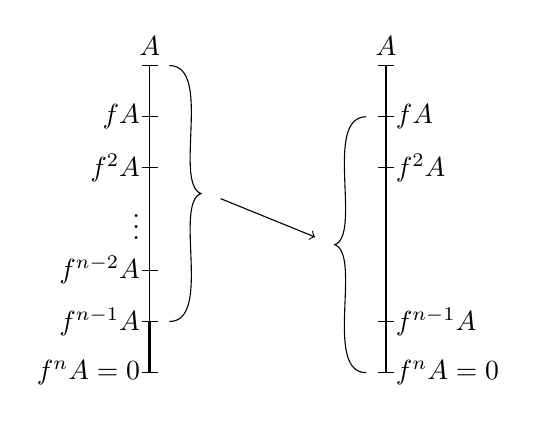
\begin{tikzpicture}[x=1cm,y=.65cm]
\draw (0,0)--(0,6);\draw[very thick] (0,0)--(0,1);
\draw (3,0)--(3,6);
\foreach \y in {0,1,2,4,5,6}{\draw (-.1,\y)--(.1,\y);}
\foreach \y in {0,1,4,5,6}{\draw (2.9,\y)--(3.1,\y);}
\node[above] at (0,6){$A$};\node[left] at (0,5){$fA$};\node[left] at (0,4){$f^2A$};\node[left] at (0,3){$\vdots$};\node[left] at (0,2){$f^{n-2}A$};\node[left] at (0,1){$f^{n-1}A$};\node[left] at (0,0){$f^nA=0$};
\node[above] at (3,6){$A$};\node[right] at (3,5){$fA$};\node[right] at (3,4){$f^2A$};\node[right] at (3,1){$f^{n-1}A$};\node[right] at (3,0){$f^nA=0$};
\draw (.25,6) .. controls (.8,6) and (.3,3.7) .. (.65,3.5) .. controls (.3,3.3) and (.8,1) .. (.25,1);
\draw (2.75,5) .. controls (2.2,5) and (2.7,2.7) .. (2.35,2.5) .. controls (2.7,2.3) and (2.2,0) .. (2.75,0);
\draw[->] (.9,3.4)--(2.1,2.65);
\end{tikzpicture}}

\figure{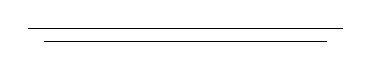
\begin{tikzpicture}\draw (0,0)--(4,0);\draw (.2,-.17)--(3.8,-.17);\end{tikzpicture}}
\margin{\uline{Terminologie}: Obj $A$ de \deleted{\unsure{tors.}}, de \deleted{\unsure{longueur}} \inserted{\unsure{rg}} $n$}

Supposons que l'on ait sur $\mathcal C$ une fonction \unsure{à} valeurs entières, additif pour les extensions, et qui est nulle ssi l'argument est nul. Alors ces conditions impliquent que
$\operatorname{rg}(A)=n\operatorname{rg}(A/fA)$.

\deleted{Un hom} Si $B$ est \deleted{\unsure{comme $A$}}, \deleted{\unsure{muni}} de $g$, \deleted{$B$} satisfait les conditions analogues pour $(g,n)$,
\deleted{\unsure{donc}} et si $u:A-B$ est un hom compatible aux $f,g$, \deleted{\unsure{et}} si on suppose que $\operatorname{rg}(A/fA)=\operatorname{rg}(B/gB)$, alors

Conditions équivalentes

(i) $u$ est \unsure{monomorphisme}

\unsure{(i bis)} $u$ \unsure{un épimorphisme}

\unsure{(i ter)} $u$ \unsure{un isomorphisme}

\diagram{\begin{array}{lll}
\unsure{\text{(ii)}}&\operatorname{gr}^0(u)\text{ est un}&\left\{\begin{array}{l}\unsure{\text{monomorphisme}}\\\text{épimorphisme}\\\text{isomorphisme}\end{array}\right.\\
\unsure{\text{(ii bis)}}&\unsure{\operatorname{gr}^0(u)}&\unsure{\Longrightarrow}\\
\unsure{\text{(iii bis)}}&\unsure{\operatorname{gr}^i(u)}&\unsure{\Longrightarrow}
\end{array}}
\margin{\deleted{$\unsure{R_D}$} \unsure{déf. rg d'obj de BT}$=\operatorname{rg}(A/fA)$}
\margin{$\unsure{\frac{p\times\ell}{e}x=\left[\frac{p\times\ell}{e}(x)\right]}$}
\margin{\unsure{$\varphi$|$\ell$}\quad\unsure{$\frac{\ell}{e}\longleftarrow\frac{R_D}{e}x$}}
\scanpage{101}
% Archive foliation: 102. Reused unrelated typescript; printed page 51, not an author's manuscript page number.
\begin{center}-- 51 --\hfill n\textsuperscript{o} 380\end{center}
3. \uline{Sous-algèbres de} $\mathcal B(\Omega)$.

Soient $\Omega$ un espace topologique et $R$ une relation d'équivalence dans $\Omega$. On notera $T'(R)$ la sous-algèbre fermée involutive de $\mathcal B(\Omega)$ constituée par les fonctions continues bornées $f$ sur \qquad qui sont constantes sur les classes de $R$. Cette sous-algèbre $T'(R)$ est l'image de l'algèbre $\mathcal B(\Omega/R)$ par l'isométrie $q^{\mathcal B}:\mathcal B(\Omega/R)\,\mathcal B(\Omega)$ que définit l'application quotient $q:\Omega\longrightarrow\Omega/R$. D'autre part, pour toute sous-algèbre $A$ de $\mathcal B(\Omega)$, on notera $T(A)$ la relation d'équivalence dans $\Omega$ constituée par les couples $(t,t')\in\Omega^2$ tels que $f(t)=f(t')$ pour tout $f\in A$. Il est clair que le graphe de $T(A)$ est fermé. La relation d'équivalence $T(A)$ n'est pas nécessairement fermée. On a cependant le Lemme suivant :

LEMME 2.-- \uline{Pour toute sous-algèbre} $A\subset\mathcal B(\Omega)$, \uline{le saturé d'une partie compacte de} $\Omega$ \uline{pour la relation d'équivalence} $T(A)$ \uline{est fermé}.

Soit en effet $t$ un point de $\Omega$ adhérent au saturé d'un compact $K\subset\Omega$. Pour toute fonction $f\in A$ et tout $\varepsilon>0$, le voisinage fermé saturé de $f$ constitué par les points $t'\in\Omega$ tels que $|f(t)-f(t')|\leq\varepsilon$ rencontre $K$. Puisque $K$ est compact, l'intersection de ces voisinages (lorsque $f$ parcourt $A$ et que $\varepsilon$ parcourt l'ensemble des nombres réels $>0$) rencontre $K$. Cette intersection étant la classe d'équivalence de $t$, ceci prouve que $t$ appartient au saturé de $K$.

Il est évident que
\[
T'(T(A))\supset A
\]
\[
T(T'(R))\supset R
\]
pour toute sous-algèbre $A$ de $\mathcal B(\Omega)$ et toute relation d'équivalence $R$ sur $\Omega$.

PROPOSITION 4.-- \uline{Si} $\Omega$ \uline{est normal et si} $R$ \uline{est une relation d'équivalence fermée sur} $\Omega$, \uline{alors} $T(T'(R))=R$.

En effet, on sait que $\Omega/R$ est dans ce cas normal (Top. Gén., Chap.9, \S\ 4, exer.15).
\scanpage{102}
% Archive foliation: 103. Mirror blue show-through belongs to the reverse typescript.
\unsure{(iii)} $\operatorname{gr}u$ est un isom.

\[
\begin{aligned}
u\text{ mono}&\Longrightarrow\operatorname{gr}^0(u)\text{ un mono},&\text{car }\operatorname{gr}^0(u)&\simeq(f^{n-1}A-f^{n-1}B)\\
u\text{ épi}&\Longrightarrow\operatorname{gr}^0(u)\text{ un épi},&\text{car }\operatorname{gr}^0(u)&\simeq(A/fA-B/fB)
\end{aligned}
\]
\[
\operatorname{gr}^0(u)\text{ un mono}\Longleftrightarrow\operatorname{gr}^0(u)\text{ un épi}\Longleftrightarrow\operatorname{gr}^0(u)\text{ un isom}
\]
car $A/fA$ et $B/fB$ de \uline{$=\unsure{\operatorname{rg}}$}.

\[
\operatorname{gr}^0(u)\text{ un isom}\Longrightarrow\operatorname{gr}(u)\text{ un isom}
\]
\margin{car $\operatorname{gr}^i(u)\simeq(\operatorname{gr}^0(u))$ si $0\leq i\leq n-1$}
\[
\operatorname{gr}(u)\text{ un isom}\Longrightarrow u\text{ un isom}.
\]
\margin{bien connu.}

\uline{Cor.} \deleted{\unsure{Soit}} Pour \unsure{$\forall$} entier $0\leq i\leq n$, $f^iA$ est le seul sous-objet de \unsure{T.A} \inserted{$B$} de $A$, de hauteur $n-i$ et de rang $\rho$ : en effet, un tel $B$ est contenu dans $f^iA=\operatorname{Ker}f^{n-i}$, et d'après ce qui précède, lui est égal.

\uuline{Cor.} dual : $A/f^{n-i}A$ est le seul objet quotient de $A$ qui soit de Tate, de hauteur $n-i$, de rang $\rho$.

\figure{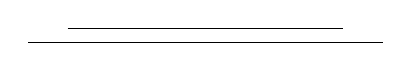
\begin{tikzpicture}\draw (0,0)--(3.5,0);\draw (-.5,-.18)--(4,-.18);\end{tikzpicture}}

$G$ schéma en groupes commutatifs, plat \deleted{\unsure{loc}} de présentation finie sur $S$. Un endom $f$, et entier $n$ tel que $f^n=0$. Soit $1\leq j\leq n-1$ fixé.

Conditions équivalentes

(i) [$\operatorname{Ker}f^j$ est plat, et] \deleted{\unsure{morphisme}} $f^{n-j}:G-\operatorname{Ker}f^j$ est fid \deleted{plat}.

(ii) $\forall s\in S$, $(G_s,f)$ est un objet de \unsure{T.A} de \deleted{\unsure{long}} hauteur $n$ (dans la catégorie des groupes algébriques commut sur $k$).
\scanpage{103}
% Archive foliation: 104, inverted at upper right. Reused unrelated typescript; printed page 47.
\begin{center}-- 47 --\hfill n\textsuperscript{o} 380\end{center}
\begin{center}\S\ 4. \uuline{Algèbres de fonctions}.\end{center}
1. \uline{Algèbres de fonctions continues bornées}.

Etant donné un espace topologique $\Omega$, on note $\mathcal B(\Omega)$ l'algèbre sur $\mathbb C$ des fonctions \inserted{continues} bornées sur $\Omega$ à valeurs dans $\mathbb C$. C'est une algèbre commutative semi-simple. L'application de $\mathcal B(\Omega)$ dans $\mathcal B(\Omega)$ qui transforme chaque fonction $f$ en la fonction conjuguée $\bar f$ est une involution de $\mathcal B(\Omega)$. On définit une norme sur $\mathcal B(\Omega)$ en posant $\lVert f\rVert=\underset{t\in\Omega}{\operatorname{Sup}}|f(t)|$ pour tout $f\in\mathcal B(\Omega)$. Cette norme est compatible avec la structure d'algèbre. Munie de cette norme, $\mathcal B(\Omega)$ est une algèbre normée complète. L'involution $f\longrightarrow\bar f$ est une isométrie. Pour tout élément $f$ hermitien, c'est-à-dire pour toute fonction bornée continue réelle, $1+f^2$ est inversible dans $\mathcal B(\Omega)$. Par suite la transformation de Gelfand de $\mathcal B(\Omega)$ vérifie la condition $\widehat{\bar f}=\overline{\hat f}$. (Prop.10). Il en résulte que l'image de la transformée de Gelfand de $\mathcal B(\Omega)$ est une sous-algèbre dense dans $\mathcal C(\operatorname{Sp}(\mathcal B(\Omega)))$ (Prop.10, Cor.\quad). Mais d'autre part, on a $\lVert f^2\rVert=\lVert f\rVert^2$ pour tout $f\in\mathcal B(\Omega)$ et par suite la transformation de Gelfand est une isométrie. On voit donc que la transformation de Gelfand est un isomorphisme isométrique de $\mathcal B(\Omega)$ sur $\mathcal C(\operatorname{Sp}(\mathcal B(\Omega)))$.

Si $\varphi$ est une application continue de l'espace $\Omega$ dans un espace $\Omega'$, on définit un homomorphisme $\varphi^{\mathcal B}$ de $\mathcal B(\Omega')$ dans $\mathcal B(\Omega)$ en posant $\varphi^{\mathcal B}(f)=f\circ\varphi$ pour tout $f\in\mathcal B(\Omega')$. Cet homomorphisme est continu car $\lVert\varphi^{\mathcal B}(f)\rVert\leq\lVert f\rVert$ pour tout $f\in\mathcal B(\Omega')$.

Pour tout $t\in\Omega$, l'application $\xi_t$ de $\mathcal B(\Omega)$ dans $\mathbb C$ définie par $\xi_t(f)=f(t)$ quel que soit $f\in\mathcal B(\Omega)$ est un caractère de $\mathcal B(\Omega)$. L'application $t\longrightarrow\xi_t$ est une application continue qui sera appelée l'application canonique de $\Omega$ dans le spectre de $\mathcal B(\Omega)$.

Pour que cette application soit injective, il faut et il suffit que $\mathcal B(\Omega)$
\scanpage{104}
% Archive foliation: 105.
\uline{Dém.} On a (i)$\Longrightarrow$(ii), car (i) implique que $\operatorname{Ker}f_s^j=\operatorname{Im}f_s^{n-j}$, et on conclut par le lemme préliminaire.

\deleted{\unsure{(i)$\Longrightarrow$(ii)}} (ii)$\Longrightarrow$(i), on a $H=\operatorname{Ker}f^j$, considérons $G\xrightarrow{g}H$ induit par $f^{n-j}$ (existe, car $f^n=0$ i.e. $f^j(f^{n-j})=0$). Par hyp. (ii), il est \inserted{fid} plat par fibre. Comme $G$ est plat de prés. finie sur $S$ et $H$ de prés. finie sur $S$, on en conclut que $g$ est \inserted{fid} plat \uline{et} $H$ est plat.

\uline{Cor.} Ceci ne dépend pas du choix de $j$, et implique que \deleted{\unsure{les $\operatorname{Ker}f^j/\operatorname{Ker}f^{j'}$ existent donc}} \inserted{les $\operatorname{Ker}f^j$ sont plats}, \deleted{\unsure{et que}} pour $j\geq j'$ $\operatorname{Ker}f^j/\operatorname{Ker}f^{j'}$ est représentable comme schém. en groupes de type fini, et $f$ dans $\mathcal C$ faisceaux \deleted{\unsure{plats}} fppf \deleted{\unsure{sur}} \inserted{\unsure{plats}} \unsure{vérifie les} conditions de Tate de hauteur $n$.

Cas $G$ fini sur $S$ : rang de Tate en un pt.
\margin{(loc. cte)}
Il y a un seul sous-objet de \unsure{T.A} de hauteur donnée $i\leq n$, de $=$ rang $\rho$.

Kif-kif pour quotients.
\scanpage{105}
% Archive foliation: 106. Reused unrelated typescript; printed page 19, n°382.
\begin{center}-- 19 --\hfill n\textsuperscript{o} 382\end{center}
de $a$ ; si $Z(f,g)$ désigne l'ensemble des points vérifiant ces conditions, $Z(f,g)$ est \uline{ouvert et fermé} dans $U$ ; en particulier, si $U$ est connexe, $Z(f,g)$ est soit vide, soit égal à $U$ (``principe du prolongement analytique'').

3.6 -- \uline{Critères d'analyticité}.

3.6.1. Supposons que $K=\underline{\underline{R}}$. Soit $U$ un ouvert de $\underline{\underline{R}}^n$ et soit $f$ une application de $U$ dans $E$. Les deux conditions suivantes sont équivalentes :

(1) $f$ est \uline{analytique} dans $U$.

(2) $f$ est \uline{indéfiniment différentiable} dans $U$ (cf. n\textsuperscript{o} 2.3.1) et pour toute partie compacte $F$ de $U$, il existe des nombres réels $C$ et $M$ tels que
\[
\lVert\Delta^s f(x)\rVert\leq C.M^{|s|}\qquad\text{si }x\in F,\quad s\in\underline{\underline{N}}^n.
\]

3.6.2. Supposons que $K=\underline{\underline{C}}$. Toute application \uline{dérivable} d'un ouvert $U$ de $\underline{\underline{C}}^n$ dans $E$ est \uline{analytique} dans $U$.

\begin{center}-:-:-:-\end{center}
\scanpage{106}
% Archive foliation: 107.
$G'\subset G\subset G''$

\diagram{\begin{array}{ccccccccc}
0&-&G'_2&\subset&G_2&\longrightarrow&G''_2&-&0\\
&&\begin{tikzpicture}[baseline=-2pt]\draw (0,.35)--(0,-.2)..controls (0,-.45) and (.16,-.4)..(.22,-.16);\end{tikzpicture}\ \alpha'&&\begin{tikzpicture}[baseline=-2pt]\draw (0,.35)--(0,-.2)..controls (0,-.45) and (.16,-.4)..(.22,-.16);\end{tikzpicture}\ \alpha&&\begin{tikzpicture}[baseline=-2pt]\draw (0,.35)--(0,-.2)..controls (0,-.45) and (.16,-.4)..(.22,-.16);\end{tikzpicture}\ \alpha''&&\\
0&\longrightarrow&G'_1&\subset&G_1&\longrightarrow&G''_1&-&0
\end{array}}
\margin{\deleted{$0-\operatorname{Ker}\unsure{G''_1}\longrightarrow$}}

$p:G_2-G_2$ se factorise à travers $G_1$, et s'annule sur $G_1$, induit un isom
\[
G_2/G_1\xrightarrow{\sim}G_1
\]
$p:G'_2-G'_2$ se factorise à travers $G'_1$ (\deleted{\unsure{sur}} \unsure{on} \unsure{OK} sur fibre gén.), et s'annule sur $G'_1$ ($=$ raison) donc induit
\[
G'_2/G'_1\xrightarrow{\sim}G'_1
\]
\diagram{\begin{array}{ccc}
G'_2&\subset&G_2\\
\vert&&\begin{tikzpicture}[baseline=-2pt]\draw (0,.35)--(0,-.2)..controls (0,-.45) and (.16,-.4)..(.22,-.16);\end{tikzpicture}\\
G'_1&\subset&G_1
\end{array}}
\[
\operatorname{Ker}\alpha''\simeq(\underbrace{G'_2\cap G_1}_{\operatorname{Ker}p_{G'_2}})/G'_1\simeq\operatorname{Ker}(G'_2/G'_1\longrightarrow G'_1)
\]
\[
G'_2=\overline{G'_{2\eta}}
\]
\[
G'_1=\overline{G'_{1\eta}}=\overline{G'_{2\eta}\cap G_{1\eta}}\subset\overline{G'_{2\eta}}\cap\overline{G_{1\eta}}=\overset{\deleted{\unsure{\sim}}}{G'_{2\unsure{\eta}}}\cap G_1=\operatorname{Ker}(p_{G'_2})
\]
\margin{\fbox{égalité ssi $G'_2\cap G_1$ plat/$S$}}

\unsure{La question donc est} \uline{$\operatorname{Ker}\alpha''$}, qui est un \unsure{groupe} \deleted{\unsure{fid...}} \unsure{fini}.

\diagram{\begin{tikzcd}[column sep=small]
0\arrow[r,no head]&\operatorname{Ker}\alpha''\arrow[r]&G'_2/G'_1\arrow[r]\arrow[d,phantom,"\rotatebox{90}{$\simeq$}" description]\arrow[ddr,no head]&G_2/G_1\arrow[r]\arrow[d,phantom,"\rotatebox{90}{$\simeq$}" description]&G''_2/\operatorname{Im}G''_1\arrow[r]&0\\
&&\widetilde{G'_1}&G_1&&\\
&&&G'_1\arrow[u]&&
\end{tikzcd}}
\scanpage{107}
% Archive foliation: 108.
? \uline{Proof of 1\textsuperscript{st} conj.} :

\textcircled{1} Given
\[
0\longrightarrow\Phi'\longrightarrow\Phi(G)\longrightarrow\Phi''\longrightarrow0
\]
(Galois-devissage), then can define $G'$, $G''$
so $\Phi'=\Phi(G')$, \uline{$\Phi''=\Phi(G'')$}

\deleted{$\unsure{f^j x-fy}$}
\[
\begin{array}{cccc}
f^j x=0&x=fy&x=f^2z&x=f^{n-j\unsure{-1}}t\\
&f^{j+1}y=0&y=fz&f^{n-1}t=0\\
&&f^{j+2}z=0&
\end{array}
\]
\[
\operatorname{Ker}f^j=\operatorname{Im}\qquad
\operatorname{Ker}f=\operatorname{Im}f^{n-1}
\]
\margin{$\supset$ \unsure{triv.}\quad $\subset$ hyp}
\diagram{\begin{tikzcd}
\operatorname{Ker}f^j=\operatorname{Im}f^{n-j}\arrow[d,Rightarrow,"?"]\\
\operatorname{Ker}f^{j+1}=\operatorname{Im}f^{n-j-1}
\end{tikzcd}}
\[
f^{j+1}x=0\qquad
\left\{\begin{array}{l}fx\in\operatorname{Ker}f^j\\fx=f^{n-j}y\end{array}\right.
\]
\[
\unsure{f^{-1}}(\deleted{\unsure{f}}\inserted{f^{n-j}}A)=f^{n-j-1}A
\]

\margin{
\diagram{\begin{tikzcd}
\operatorname{Ker}f^j=\operatorname{Im}f^{n-j}\arrow[d,Rightarrow]\\
\operatorname{Ker}f^{j-1}=\operatorname{Im}f^{n-j\unsure{+1}}
\end{tikzcd}}
$f^{j-1}x=0\Longrightarrow f^j x=0\qquad x=f^{n-j}y\quad\deleted{\unsure{f}}$
$f^{j-1}x=f^{n-1}y=0$
i.e. $f^j(\overbrace{f^{n-1-j}y}^{f^{n-j}z})=0$
\deleted{$\unsure{f^{n-j}y=0}$}
}

\margin{
$n=3\qquad f^3=0$
\[
\operatorname{Ker}f=\operatorname{Im}f^2
\]
$f^{j-1}x=0\qquad f^j x=0\qquad x=fy\qquad f.$
\[
A/f^2A\xrightarrow[\sim]{f}fA
\]
\[
fA/f^2A\xrightarrow{\sim}f^2A
\]
\deleted{$\unsure{A/fA}$}
\[
(f^j)^{-1}(f^{n-1}(A))=fA
\]
$\operatorname{Ker}f^j$
}

\figure{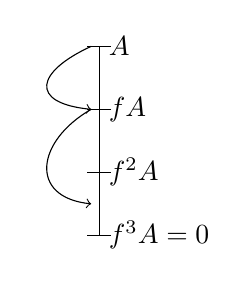
\begin{tikzpicture}[x=1cm,y=.8cm]
\draw(0,0)--(0,3);\foreach \y in {0,1,2,3}{\draw(-.15,\y)--(.15,\y);}
\node[right]at(0,3){$A$};\node[right]at(0,2){$fA$};\node[right]at(0,1){$f^2A$};\node[right]at(0,0){$f^3A=0$};
\draw[->](-.1,3)..controls(-.8,2.6)and(-.9,2.1)..(-.1,2);
\draw[->](-.1,2)..controls(-.8,1.5)and(-.9,.6)..(-.1,.5);
\end{tikzpicture}}

\figure{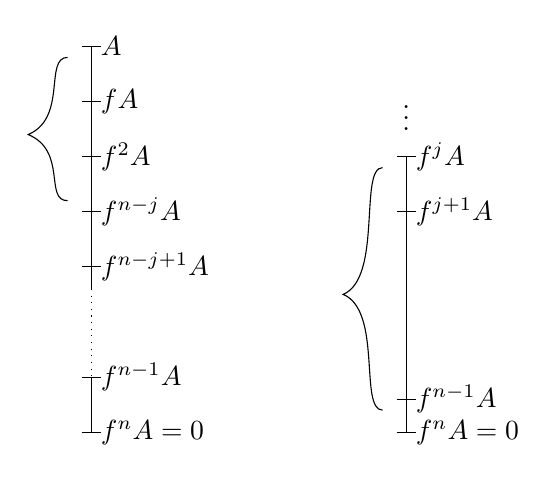
\begin{tikzpicture}[x=1cm,y=.7cm]
\draw(0,7)--(0,3);\draw(0,3)--(0,2.6);\draw[dotted](0,2.6)--(0,1);\draw(0,1)--(0,0);
\foreach \y in {0,1,3,4,5,6,7}{\draw(-.12,\y)--(.12,\y);}
\node[right]at(0,7){$A$};\node[right]at(0,6){$fA$};\node[right]at(0,5){$f^2A$};\node[right]at(0,4){$f^{n-j}A$};\node[right]at(0,3){$f^{n-j+1}A$};\node[right]at(0,1){$f^{n-1}A$};\node[right]at(0,0){$f^nA=0$};
\draw(-.3,6.8)..controls(-.6,6.8)and(-.3,5.7)..(-.8,5.4)..controls(-.3,5.1)and(-.6,4.2)..(-.3,4.2);
\draw(4,0)--(4,5);\foreach \y in {0,.6,4,5}{\draw(3.88,\y)--(4.12,\y);}
\node[above]at(4,5.3){$\vdots$};\node[right]at(4,5){$f^jA$};\node[right]at(4,4){$f^{j+1}A$};\node[right]at(4,.6){$f^{n-1}A$};\node[right]at(4,0){$\unsure{f^nA=0}$};
\draw(3.7,4.8)..controls(3.4,4.8)and(3.7,2.8)..(3.2,2.5)..controls(3.7,2.2)and(3.4,.4)..(3.7,.4);
\end{tikzpicture}}
\scanpage{108}
% Archive foliation: 109.
\uline{Conditions équivalentes}

a) $G'_1=G'_2\cap G_1\quad(=\operatorname{Ker}p_{G'_2})$

b) $G'_2\cap G_1$ est plat/$S$

c) $G'_2$ est un gpe de Tate de hauteur $2$

d) $G'_2/G'_1\xrightarrow{\text{induit par }p}G'_1$ est \deleted{\unsure{un mono épi}} un mono

e) $G'_2/G'_1\xrightarrow{\text{induit par }p}G'_1$ est un \uline{épim.}

\deleted{\unsure{g)}}\inserted{f)} $G'_2\xrightarrow{p}G'_1$ est un \uline{épim.}

$f^*$\deleted{\unsure{bis}}) $G''_1\longrightarrow G''_2$ un mono.

$e^*$) \deleted{$\unsure{G''_2}$} $\operatorname{Ker}(G''_2\xrightarrow[\text{épim}]{p}G''_1)\longleftarrow G''_1$ un mono.

$d^*$) id un épim.

$c^*$) $G''_2$ est un gpe de Tate de hauteur $2$

$b^*$) $\ldots$

$a^*$) $\ldots$

\figure{\begin{tikzpicture}\draw(0,0)--(10,.5);\draw(-.5,0)--(-2,-1.5)--(-2,-5.5);\draw(-1.8,-5.5)--(10,-5.5);\end{tikzpicture}}
\[
(\mathbb Z/p^2\mathbb Z\times\mathbb Z/p^2\mathbb Z)_\eta\simeq G_{2\eta}
\]
\margin{$G_{2s}$ purement infinitésimal. et unipotent}
\[
\mathbb Z/p^2\mathbb Z\qquad G'_\eta\xrightarrow{p}G'_\eta\qquad G'_s\xrightarrow{p}G'_s
\]
\[
\mathbb Z/p^2\mathbb Z\longrightarrow\alpha_p^{\unsure{2}}
\]
\margin{\deleted{\unsure{On}}}
\figure{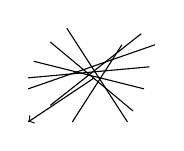
\begin{tikzpicture}[scale=.7]
\draw(-1.2,0)--(1,.2);\draw(-1.1,.3)--(.9,-.2);\draw(-.8,.65)--(.7,-.6);\draw(-.5,.9)--(.6,-.8);\draw(-.8,-.5)--(.85,.8);\draw(-.4,-.8)--(.5,.6);\draw(-1.2,-.2)--(1.1,.6);\draw[->](0,0)--(-1.2,-.8);\end{tikzpicture}}

\diagram{\begin{tikzcd}C\arrow[r,"u"]&C\end{tikzcd}}
$u_s=F$

\diagram{\begin{tikzcd}
C\arrow[r,no head,"F"]&C\\
C\arrow[u,phantom,"\sim" description]\arrow[ur,"V"']&
\end{tikzcd}}

\diagram{\begin{tikzcd}
C\arrow[r,"F"]\arrow[rr,bend right,"p"']&C^{(p)}\arrow[r,no head,"V"]&C
\end{tikzcd}}
\deleted{$C\longrightarrow C^{(p)}$}

$VF=p\qquad\unsure{C=C^{(p^2)}|C=C^{(p)}}$
\margin{\unsure{?}}
\margin{$F\quad\vert\qquad\deleted{F}\quad FV=p$}

$\unsure{E_2}\qquad V=uF\qquad V^2=up$

$F=u^{-1}V\qquad F^2=u^{-1}p$

\deleted{$\unsure{VF=u}$}
\scanpage{109}
% Archive foliation: 110. Reused unrelated typescript; printed page 18, n°382.
\begin{center}-- 18 --\hfill n\textsuperscript{o} 382\end{center}
\[
f(a+h)=\sum\Delta^s f(a).h^s\qquad\text{si $h$ est assez petit.}
\]
Soit $C_E^\omega(U)$ l'espace vectoriel des applications analytiques de $U$ dans $E$. Les $\Delta^s$ sont des endomorphismes $K$-linéaires de $C_E^\omega(U)$. On a
\[
\Delta^s\circ\Delta^t=\Delta^{s+t}.
\]
De plus, avec les notations et hypothèses du n\textsuperscript{o} 3.4.2., on a
\[
\Delta^s(f^1.f^2)=\sum_{u+v=s}\Delta^u f^1.\Delta^v f^2.
\]

3.5.3. Soit $f$ une application analytique d'un ouvert $U$ de $K^n$ dans $E$, et soit $g$ une application analytique d'un ouvert $V$ de $K^m$ dans $U$. L'application composée $f\circ g$ est analytique. En outre, supposons que $0\in V$ et que $g(0)=0$. Le développement de $f\circ g$ en série entière au point $0$ s'obtient alors en substituant, dans le développement de $f$ au point $0$, les développements en série entière des composantes $g_i$ de $g$ au point $0$ (cf. n\textsuperscript{o} 3.4.4.).

3.5.4. Soit $f=\sum b_s x^s$ une série convergente à coefficients dans $E$, et soit $D(f)$ son domaine de convergence stricte. La fonction définie par $f$ sur $D(f)$ est analytique. Pour tout $s\in\underline{\underline{N}}^n$, on a
\[
\Delta^s f(x)=\sum\binom{s+t}{s}b_{s+t}x^t,
\]
la série du membre de droite ayant un domaine de convergence stricte qui contient celui de $f$ (et lui est égal si $K=\underline{\underline{R}}$ ou $K=\underline{\underline{C}}$).

3.5.5. Si $f$ est analytique dans un ouvert $U$ de $K^n$, $f$ est \uline{strictement dérivable} dans $U$ (cf. n\textsuperscript{o} 1.2.4) et ses dérivées partielles $D_i f$ sont analytiques. Les dérivées partielles itérées $D^s f$ de $f$ sont données par la formule
\[
D^s f=s!\,\Delta^s f.
\]

3.5.6. Soient $f$ et $g$ deux applications analytiques d'un ouvert $U$ de $K^n$ dans $E$. Soit $a\in U$. Pour que $f$ et $g$ aient un contact d'ordre $\geq k$ en $a$, il faut et il suffit que $\Delta^s f(a)=\Delta^s g(a)$ si $|s|\leq k$. Pour que $f$ et $g$ aient un contact d'ordre infini en $a$, il faut et il suffit qu'elles soient égales dans un voisinage
\scanpage{110}
% Archive foliation: 111.
\[
0\longrightarrow N-G\xrightarrow{u}H\longrightarrow0\quad\not\Longrightarrow\quad\overset{\text{\inserted{\figure{\begin{tikzpicture}\node[draw,ellipse] {\unsure{formellt}};\end{tikzpicture}}}}}{\text{\uline{ker est lisse}}}
\]
\deleted{$G(\hat S)\longrightarrow H(\hat S)$}

$G\longrightarrow H$

$\Phi(G)\longrightarrow\Phi(H)$ \uline{surj.}

$G\xrightarrow{u}H$\qquad hom de gpes divisibles \unsure{sur le T.K.}

Conditions équivalentes

(i) L'hom $u(1):G(1)-H(1)$ est un \uline{épim.}
\margin{[il suffit de vérifier sur fibre spéciale]}

(ii) L'hom $u(n):G(n)-H(n)$ est un [idem] épim $\forall n$.

(iii) L'hom $u$ est \uline{formellt lisse} et un \uline{épim.}

(iii bis) L'hom $u_s:G_s-H_s$ est form\textsuperscript{t} lisse et un épim.

(iv) L'hom de gpes divisibles sur $K$ :
\[
G_{|K}-H_{|K}
\]
\deleted{\unsure{est un}} [form\textsuperscript{t} lisse et] un épim

(iv bis) $\Phi(G)-\Phi(H)$ est surjectif

\figure{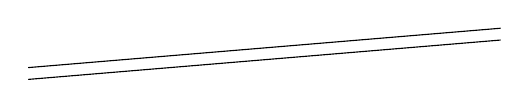
\begin{tikzpicture}\draw(0,0)--(6,.5);\draw(0,-.15)--(6,.35);\end{tikzpicture}}

\diagram{\left\{\begin{array}{ll}
a)&\text{Si }\Phi(u)\text{ est un isom, alors }u\text{ est un isom}\\
&\text{($\Phi$ est ``conservatif'')}\\
b)&\text{Si }u\text{ est déjà formellt fid. plat, }\deleted{\unsure{\Phi(u)\text{ surj}}}\\
&\text{mais pas form\textsuperscript{t} lisse [i.e. Ker }u\text{ pas form\textsuperscript{t} lisse]}\\
&\text{alors }\Phi(u)\text{ pas surjectif}\ldots
\end{array}\right.}
\scanpage{111}
% Archive foliation: 112, inverted at upper right. Reused unrelated typescript; printed page 15, n°382.
\begin{center}-- 15 --\hfill n\textsuperscript{o} 382\end{center}
qu'il existe un nombre réel $M$ tel que
\[
\lVert b_s\rVert\leq M^{|s|}\qquad\text{pour tout }s\ne0.
\]
Les séries absolument convergentes forment un sous-espace vectoriel $E\{\{X\}\}$ de $E[[X]]$ ; c'est un module sur l'algèbre $K\{\{X\}\}$ des séries convergentes scalaires. Lorsque $E$ est un espace vectoriel de dimension finie, l'application canonique de $E\otimes_K K\{\{X\}\}$ dans $E\{\{X\}\}$ est un isomorphisme.

3.3.3. Soit $f=\sum b_sX^s$ une série convergente à coefficients dans $E$. Soit $J(f)$ le sous-ensemble de $\underline{\underline{R}}_+^n$ formé des points $r=(r_1,\ldots,r_n)$, $r_i>0$, tels que la série à termes positifs $\sum\lVert b_s\rVert r^s$ soit convergente. Si $r\in J(f)$, la série $f$ est absolument convergente en tout point du polydisque $B(r)$. L'intérieur $I(f)$ de $J(f)$ s'appelle \uline{l'indicatrice de convergence} de $f$. Pour qu'un point $r=(r_1,\ldots,r_n)$, $r_i>0$, appartienne à $I(f)$, il faut et il suffit qu'il existe un point $r'=(r'_1,\ldots,r'_n)$, avec $r'_i>r_i$, tel que
\[
\operatorname{Sup}\lVert b_s\rVert r'^{s}<+\infty.
\]
Soit $\Omega(f)$ le sous-ensemble de $\underline{\underline{R}}^n$ formé des points
\[
\log r=(\log r_1,\ldots,\log r_n),
\]
où $r$ parcourt $I(f)$. C'est un sous-ensemble ouvert \uline{convexe} de $\underline{\underline{R}}^n$ ; de plus, il existe un nombre réel $k$ (dépendant de $f$) tel que $\Omega(f)$ contienne tous les points $(a_1,\ldots,a_n)$ tels que $a_i\leq k$.

3.3.4. L'ensemble $D(f)=\bigcup_{r\in I(f)}B(r)=\bigcup_{r\in J(f)}B(r)$ est un ouvert non vide de $K^n$ ; il est contenu dans l'intérieur $\overset{\circ}{C}(f)$ de l'ensemble $C(f)$ des points où $f$ converge absolument ; lorsque $K$ est égal à $\underline{\underline{R}}$ ou à $\underline{\underline{C}}$, on a $D(f)=\overset{\circ}{C}(f)$. L'ouvert $D(f)$ est appelé le \uline{domaine de convergence stricte} de $f$.

3.4 -- \uline{Opérations sur les séries convergentes}.

3.4.1. Soit $E'$ un espace vectoriel normé complet et soit $u:E\longrightarrow E'$ une application linéaire continue. Soit $f=\sum b_sX^s$ une série convergente à coefficients dans $E$. Alors la série
\scanpage{112}
% archive foliation: 113
\scanpage{113}
% archive foliation: 114
\margin{\fbox{Conférence à Nice}}
\uline{Groupes de Barsotti--Tate}
\fbox{$p$ fixé}

1) fppf sur $S$

$G$ gpe de B.T si
\[
\begin{array}{ll}
a)&pG=G\\
b)&G\text{ de $p$-torsion}\\
c)&{}_pG=\operatorname{Ker}p.\operatorname{id}_G\quad\text{fini loc. libre}
\end{array}
\]
Alors les ${}_{p^n}G=G(n)$ le sont aussi. Si $G(1)$ de rang $p^d$, alors $G(n)$ de rang $p^{nd}$ ; on a $G=\underrightarrow{\lim}_nG(n)$

Exemple important : $A$ schéma abélien,
\[
G(n)={}_{p^n}A\qquad G={}_{p^\infty}A
\]
\deleted{\unsure{2)}} Th. de Serre--Tate
\[
S_o\subset S\qquad A\longmapsto(A_o,{}_{p^\infty}A,\varphi)
\]
\margin{\deleted{\unsure{S...}} de car. $p$}
une équivalence de catégories

2) Groupe formel $\bar G$ associé à un groupe de B.T.

3) \uline{Cristaux}\qquad Puissances divisées sur un idéal $J$
\[
x^{(n)}\quad(n\geq0)\quad\left(\frac{x^n}{n!}\right)
\]
\margin{$x^{(0)}=1,\ x^{(1)}=x\qquad x^{(n)}\in J$}
\[
\left\{\begin{array}{l}
(x+y)^{(n)}=\displaystyle\sum_{i+j=n}x^{(i)}x^{(j)}\\[1em]
(\lambda x)^{(n)}=\lambda^n x^{(n)}\\[2em]
\ldots
\end{array}\right.
\]
\margin{$J^{(n)}$ \inserted{idéal} engendré par les monômes de poids $\geq n$ en les $x^{(i)}$ ($x\in J$)}

\deleted{\uuline{Site cristallin absolu}\quad$\{$\quad$\unsure{x}$}

puiss. div. nilpotentes : $J^{(n)}=0$ si $n$ grand

\rule{2cm}{.3pt} quasi nilpotentes : $J^{(n)}$ de torsion pour $n$ grand

i.e. $(n-1)!J^{(n)}=0$

exponentielle
\[
\exp(x)=\sum_{n\geq0}x^{(n)}\qquad\text{OK. si p.d. nilp.}
\]
\[
\log(1+x)=\sum_{n\geq1}(-1)^{n-1}(n-1)!x^{(n)}\qquad\text{OK.}\quad\rule{1cm}{.3pt}\quad\text{quasi-nilp.}
\]
\margin{\unsure{début de} Théorie cohomologique \unsure{développée par} Berthelot (et Illusie)}

\uline{Site cristallin} \deleted{\unsure{naturel|relatif}} \inserted{(absolu)}\quad\deleted{\unsure{cris}}

\unsure{nilpot. au sens Berthelot} (\unsure{si} $p$ nilp sur $S$)

On exige que les p.d. de $p$ soient les habituelles $\ldots$
\scanpage{114}
% archive foliation: 115
Cristaux de Modules \{loc. libres\} $=$ Modules loc. libres sur le site cristallin

\uline{Ex. 1}\quad $S$ \deleted{schéma} \inserted{$=\operatorname{Spec}A_o$, $A_o$ anneau} parfait de car $p>0$.

$A=W(A_o)$, alors les cristaux sur $A_o$ sont les Modules loc. libres sur $A$

\uline{Ex. 2}\quad $X_o$ lisse sur corps parfait $k$, $W=W(k)$,
$\mathfrak X$ remontant $X_o$ en schéma \inserted{formel} lisse sur $W$,
\deleted{[\unsure{et} $F:X-X$ remontant \unsure{Frobenius} en un hom $\unsure{\sigma_W|\varphi_W}$-linéaire de $X$]}
Un cristal est un module loc. libre $M$ sur $\mathfrak X$, muni connexion à courbure nulle rel/$W$.

Ce sont des \unsure{genres|germes} d'animaux \deleted{\unsure{dans}} rencontrés anciennement par Dwork, Katz, $\ldots$
\deleted{\unsure{Monsky}}

\figure{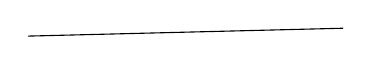
\begin{tikzpicture}\draw(0,0)--(4,.1);\end{tikzpicture}}
4)

I) $S$ schéma avec $p$ loc nilpotent. On définit ``foncteur de Dieudonné''
\[
\mathrm{BT}(S)^o\longrightarrow\mathrm{Cris}\,\mathrm{mod}\,\mathrm{loclib}(S)
\]
\[
G\longmapsto\mathbf D(G)
\]
\margin{compatible aux chgt. de base}

II) \deleted{Soit} $S$ de car. $p$, alors $M=\mathbf D(G)$ est muni de $F_M,V_M$ avec
\[
F_MV_M=p.\operatorname{id},\qquad V_MF_M=p\operatorname{id}
\]
i.e. $D(G)$ est un cristal de Dieudonné.

Il se pourrait que le foncteur \unsure{!}
\[
\mathrm{BT}(S)^o\longrightarrow\mathrm{Cris}\,\mathrm{Dieud}(S)
\]
soit pl. fidèle, et j'ai une idée de ce qui pourrait être l'image essentielle
\scanpage{115}
% archive foliation: 116
\overline{\underline{\mathrm{III}}}) Dans le cas où $S=\operatorname{Spec}(k)$, $k$ corps parfait de car. $p>0$, on retrouve le foncteur de Dieudonné habituel.

\overline{\underline{\mathrm{IV}}}) (Déformations) $D(G)_S$ est filtré par
\[
0\longrightarrow\overset{\deleted{\unsure{\vee}}}{\unsure{\omega_{G^*}}}\longrightarrow D(G)_S\longrightarrow\omega_{G^*}^{\vee}\longrightarrow0.
\]
Soit $S_o\subset S$
\margin{ép. à p. div.}
Supposons \deleted{\unsure{que}} \inserted{\unsure{que les p. div. sur $I$ sont nilpotentes}}, \unsure{ou} bien \unsure{aussi exige} $G_o$ tel que les fibres n'aient pas de comp. toroïdale, ou que les fibres de $G_o$ soient connexes. Partant de $G_o$, on trouve que prolonger $G_o$, c'est ``la $=$ chose'' que de prolonger la filtration de $D(G_o)_{S_o}$ à $D(G_o)_S$.

\overline{\underline{\mathrm{V}}}) Prenons les groupes de BT à isog. près.

Supposons $A$ séparé et complet pour la top. $(pA)$-adique ; $A_o=A/pA$. Alors foncteur
\[
G\mathrel{\unsure{\mapstochar\relbar\relbar|\longmapsto}}(G_o,\text{filtration sur }D(G_o)_A)
\]
de
\[
\mathrm{BT}_{\mathrm{isog}}(S)\longrightarrow\unsure{\mathcal C--}
\]
est pleinement fidèle.

\uline{Cas d'un anneau} \deleted{de valuation \unsure{discrète}} \inserted{local complet \unsure{noeth}, à corps résiduel} \uline{$k$ parfait de car.} $p>0$ : Groupe de B.T. est connu \inserted{(mod. isogénie)} quand on connaît $G_o$ \uline{sur} $k$ (i.e. module de Dieud. $M$ sur $k$) et une filtration sur $(M\otimes_W A)_{\unsure{p|\mathbb Q}}$
